\documentclass{beamer}

% --- Configurações de Tema ---
\usetheme{Madrid}
\usecolortheme{default}
\usepackage[portuguese]{babel}
\usepackage[utf8]{inputenc}
\usepackage{graphicx}
\usepackage{booktabs}
\usepackage{listings}
\usepackage{siunitx}
\usepackage[backend=biber, style=numeric, sorting=nty]{biblatex}
\addbibresource{referencias_numerico.bib}
\setbeamertemplate{bibliography item}{\insertbiblabel}

\lstset{
    language=Python,
    basicstyle=\ttfamily\footnotesize,  % Use monospaced font
    keywordstyle=\color{blue},          % Color for keywords
    commentstyle=\color{green},         % Color for comments
    stringstyle=\color{red},            % Color for strings
    frame=single,                       % Draw a frame around the code
    breaklines=true,                    % Wrap long lines
    showstringspaces=false              % Don't show spaces in strings
    morecomment=[s]{"""}{"""},
    morecomment=[s]{'''}{'''}
}

% --- Metadados ---
\title[Circuito RC]{Simulação Numérica de um Circuito RC}
\subtitle{Métodos de Euler, Heun e RK4}
\author[Leonardo Suarez]{Aluno: Leonardo Suarez \\ \small Professor: Dra. Cibele Ladeia Aparecida}
\institute[UFRGS]{Universidade Federal do Rio Grande do Sul \\ Instituto de Matemática e Estatística}
\date{\today}

\begin{document}

\begin{frame}
    \titlepage
\end{frame}

\begin{frame}{Sumário}
    \tableofcontents
\end{frame}

\section{Fundamentação Física}

\begin{frame}{O Problema Físico \cite{moyses_eletromag,rc_circuit}}
    \begin{itemize}
        \item Circuito série contendo uma fonte $\mathcal{E}$, um resistor $R$ e um capacitor $C$.
        \item Pela 1ª lei de Kirchhoff (lei das malhas): $V_R + V_C = \mathcal{E}$.
        \item Relação constitutiva do capacitor: $I = C \frac{dV}{dt}$.
    \end{itemize}

    Substituindo $V_R = RI$ e $I = C \frac{dV}{dt}$, obtemos a EDO:
        \begin{equation} 
            RC \frac{dV}{dt} + V = \mathcal{E}
        \end{equation}

    \begin{figure}
        \centering
        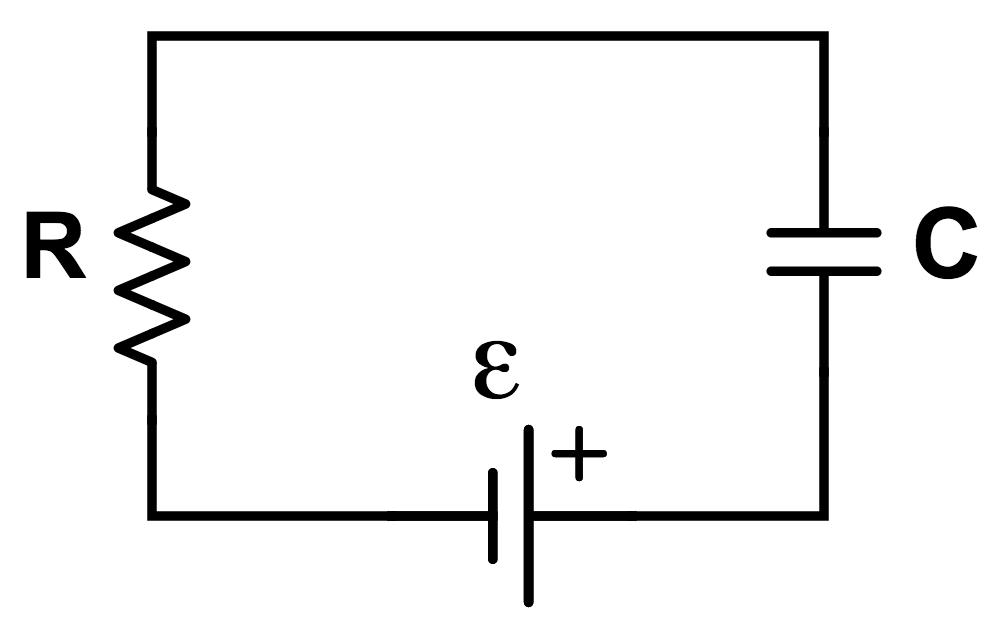
\includegraphics[width=\textwidth, height=0.4\textheight, keepaspectratio]{circuito_rc.png}
        \label{fig:circuito_rc}
    \end{figure}    
\end{frame}

\begin{frame}{O Problema de Valor Inicial (PVI)}
    Ajustando para a forma padrão $\frac{dV}{dt} = f(t, V)$:
    \begin{equation} 
        \frac{dV}{dt} = \frac{1}{RC} (\mathcal{E} - V),
    \end{equation} cuja solução analítica é dada por:
    \begin{equation}
        V(t) = \mathcal{E} \left(1 - e^{-\frac{t}{RC}}\right).
    \end{equation}
    
    \emph{Dados do problema:}
    \begin{itemize}
        \item $\mathcal{E} = \SI{10}{\volt}$
        \item $1/RC = 0.5$
        \item $V(0) = 0$ (capacitor descarregado)
    \end{itemize}
\end{frame}

\section{Métodos Numéricos}

\begin{frame}{Métodos Implementados \cite{reamat,burden}}
    Foram comparados três métodos de diferentes ordens:
    \begin{enumerate}
        \item \textbf{Euler (1ª ordem):} $V_{n+1} = V_n + h f(t_n, V_n)$
        \item \textbf{Heun (2ª ordem):} Método do trapézio/preditor-corretor.
        \item \textbf{Runge-Kutta 4ª ordem:} Média ponderada de 4 inclinações.
    \end{enumerate}
    \vspace{0.3cm}
    Analisados com passos $h \in \{1.0, 0.2, 0.05\}$.
\end{frame}

\begin{frame}[fragile]{Implementação do Método de Euler}
    \begin{lstlisting}
        def euler(f, u0, t0, tf, h):
            n = int((tf-t0)/h)
            t = np.linspace(t0, tf, n+1) # create time vector with n+1 elements (or n subintervals)
            u = np.zeros(len(t)) # start solution vector
            u[0] = u0 # set initial condition

            for k in range(0, len(t) - 1):
                u[k+1] = u[k] + h * f(t[k], u[k])
            return t, u
    \end{lstlisting}
\end{frame}

\begin{frame}[fragile]{Implementação do Método de Heun}
    \begin{lstlisting}
        def heun(f, u0, t0, tf, h):
            n = int((tf-t0)/h)
            t = np.linspace(t0, tf, n+1)
            u = np.zeros(len(t))
            u[0] = u0

            for k in range(0, len(t) - 1):
                k1 = f(t[k], u[k])
                k2 = f(t[k] + h, u[k] + h * k1)
                u[k+1] = u[k] + (h/2) * (k1 + k2)
            return t, u
    \end{lstlisting}
\end{frame}

\begin{frame}[fragile]{Implementação do Método de RK4}
    \begin{lstlisting}
        def rk4(f, u0, t0, tf, h):
            n = int((tf-t0)/h)
            t = np.linspace(t0, tf, n+1)
            u = np.zeros(len(t))
            u[0] = u0

            for k in range(0, len(t) - 1):
                k1 = f(t[k], u[k])
                k2 = f(t[k] + h/2, u[k] + (h/2) * k1)
                k3 = f(t[k] + h/2, u[k] + (h/2) * k2)
                k4 = f(t[k] + h, u[k] + h * k3)
                u[k+1] = u[k] + (h/6) * (k1 + 2*k2 + 2*k3 + k4)
            return t, u
    \end{lstlisting}
\end{frame}

\section{Resultados}

\begin{frame}{Comparação dos Métodos}
    \begin{figure}
        \centering
        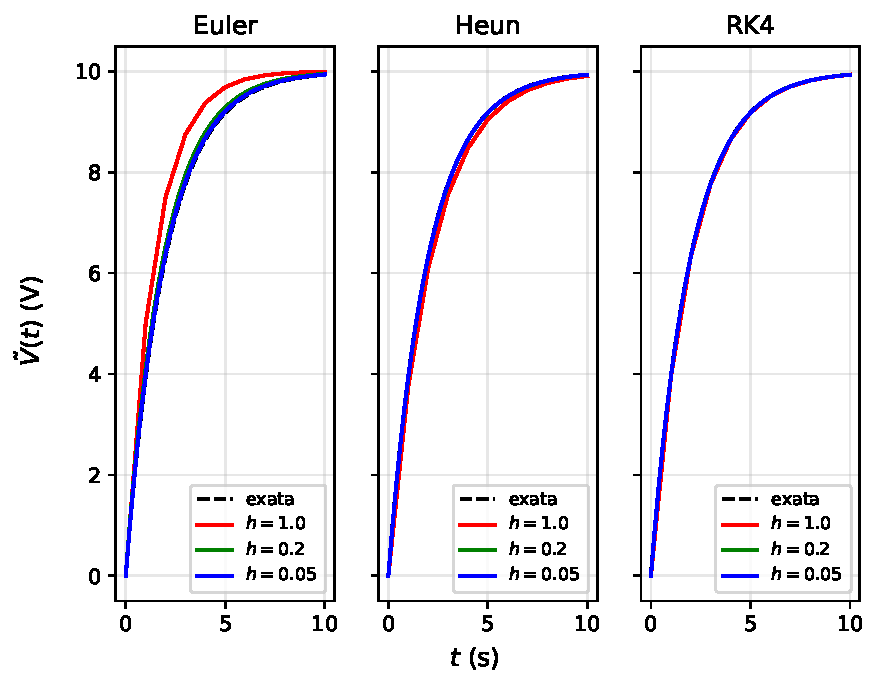
\includegraphics[width=\textwidth, height=0.8\textheight, keepaspectratio]{comparacao_metodos_edo.pdf}
        \label{fig:comparacao_metodos_edo}
    \end{figure}    
\end{frame}

\begin{frame}{Análise dos Erros}
    \begin{table}
    \centering
    \label{tab:erros}
    \footnotesize
    % Definindo a precisão e o formato de exibição
    \sisetup{
        round-mode = places,
        round-precision = 6,
        scientific-notation = true
    }
    \begin{tabular}{l c S[table-format=1.6e-1] S[table-format=1.6e-2]}
        \toprule
        Método & Passo \(h\) & {Erro Máximo} & {Erro em \(t_{\max}\)} \\
        \midrule
        Euler & 1    & 1.178794411714423e-0 & 5.761384499085409e-2 \\
        Heun  & 1    & 2.274555882855767e-1 & 2.357000018643873e-2 \\
        RK4   & 1    & 2.914030125855227e-3 & 2.672847229518993e-4 \\
        \midrule
        Euler & 0.2  & 1.920100107144238e-1 & 1.584171791765243e-2 \\
        Heun  & 0.2  & 6.615436621094872e-3 & 6.080125442835538e-4 \\
        RK4   & 0.2  & 3.332410560830112e-6 & 3.051766963579894e-7 \\
        \midrule
        Euler & 0.05 & 4.647001283561725e-2 & 4.149476121153128e-3 \\
        Heun  & 0.05 & 3.904854541776359e-4 & 3.576754513545666e-5 \\
        RK4   & 0.05 & 1.222741996542709e-8 & 1.119762060852736e-9 \\
        \bottomrule
    \end{tabular}
    \end{table}
\end{frame}

\begin{frame}{Análise dos Erros}
    \begin{figure}
        \centering
        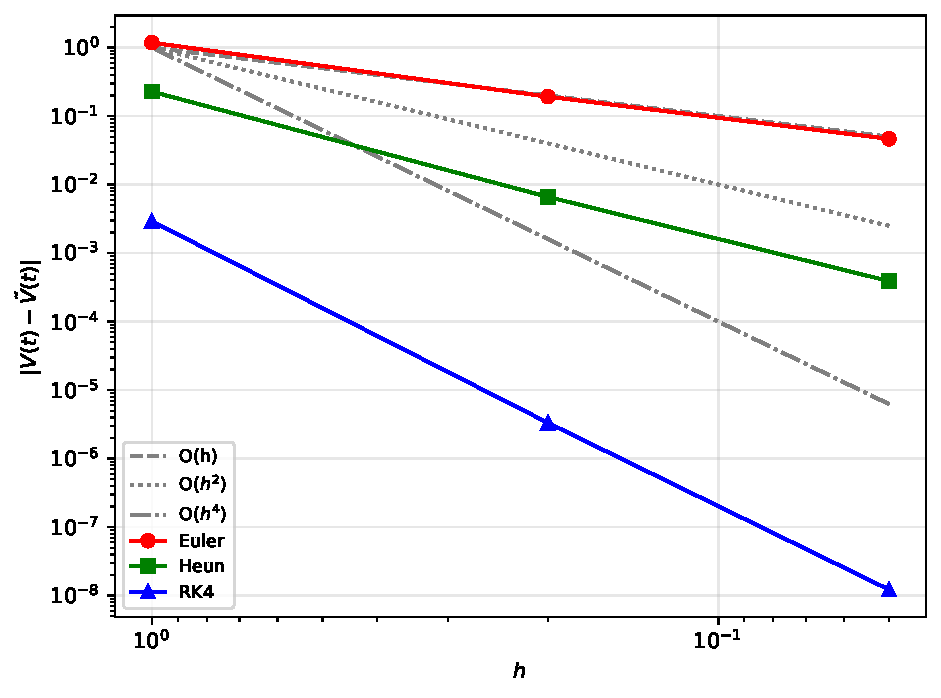
\includegraphics[width=\textwidth, height=0.8\textheight, keepaspectratio]{analise_erro_edo.pdf}
        \label{fig:analise_erro_edo}
    \end{figure}    
\end{frame}

\section{Conclusão}

\begin{frame}{Conclusão}
    \begin{itemize}
        \item RK4 com \(h=1\) (\num{10} passos) já apresenta erro máximo da ordem de \(10^{-3}\), enquanto Euler com \(h=0.05\) (200 passos) ainda tem erro da ordem de \(10^{-2}\).
        \item O erro maior ocorre próximo ao início do carregamento, onde a curvatura da solução é mais acentuada.
        \item Para os passos escolhidos, todos os métodos convergem para a solução exata, indicando que erros de arredondamento não dominaram o comportamento numérico.
    \end{itemize}
\end{frame}

\section{Referências}
    \begin{frame}{Referências Bibliográficas}
        \printbibliography
    \end{frame}

\end{document}